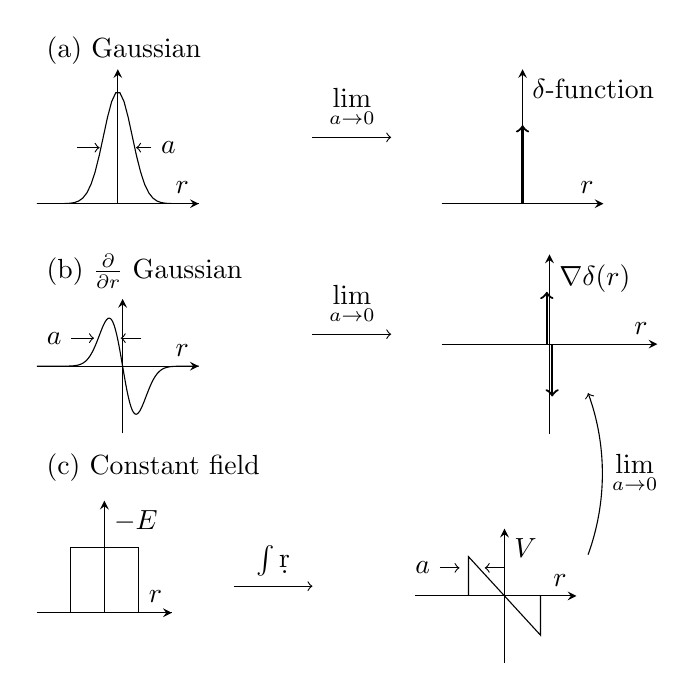
\begin{tikzpicture}

  % case (a)
  \node[anchor=west] at (0,1.8) {(a) Gaussian};

  % Gaussian
  \begin{axis}[
        xmax=4,ymax=1.2,
        xmin=-4,ymin=0,
        samples=50,
        axis lines=middle,
        ytick style={draw=none},
        xtick style={draw=none},
        yticklabels={,,},
        xticklabels={,,},
        xlabel={$r$},
        ylabel={},
        scale=0.3,
        at = {(0,-10)},
     ]
     \addplot[black] {exp(-x^2)};
     \node (a) at (axis cs:2.5,.5) {$a$};
     \draw[->] (a) -- (axis cs:.9,.5);
     \draw[->] (axis cs:-2.0,.5) -- (axis cs:-.9,.5);
  \end{axis}

  % arrow with limit
  \draw[->] (3.5,.7) -- node [midway, above] {$\lim\limits_{a\to0}$} (4.5,.7);

  % delta function
  \begin{axis}[
        xmax=4,ymax=1.2,
        xmin=-4,ymin=0,
        samples=150,
        axis lines=middle,
        ytick style={draw=none},
        xtick style={draw=none},
        yticklabels={,,},
        xticklabels={,,},
        xlabel={$r$},
        ylabel={$\delta$-function},
        scale=0.3,
        at = {(2000,-10)},
     ]
     \draw[->, thick] (axis cs:0,0) -- (axis cs:0,.7);
  \end{axis}

  % case (b)
  \node[anchor=west] at (0,-1) {(b) $\frac{\partial}{\partial r}$ Gaussian};

  % (d/dr) Gaussian
  \begin{axis}[
        xmax=4,ymax=1.2,
        xmin=-4.5,ymin=-1.2,
        samples=150,
        axis lines=middle,
        ytick style={draw=none},
        xtick style={draw=none},
        yticklabels={,,},
        xticklabels={,,},
        xlabel={$r$},
        ylabel={},
        scale=0.3,
        at = {(0,-430)},
     ]
     \addplot[black] {-2*x*exp(-x^2)};
     \node (b) at (axis cs:1.5,.5) {};
     \draw[->] (b) -- (axis cs:-.1,.5);
     \node[left] (a) at (axis cs:-2.7,.5) {$a$};
     \draw[->] (a) -- (axis cs:-1.5,.5);
  \end{axis}

  % arrow with limit
  \draw[->] (3.5,-1.8) -- node [midway, above] {$\lim\limits_{a\to0}$} (4.5,-1.8);

  % two delta functions
  \begin{axis}[
        xmax=4,ymax=1.2,
        xmin=-4,ymin=-1.2,
        samples=150,
        axis lines=middle,
        ytick style={draw=none},
        xtick style={draw=none},
        yticklabels={,,},
        xticklabels={,,},
        xlabel={$r$},
        ylabel={$\nabla\delta(r)$},
        scale=0.4,
        at = {(1500,-323)},
     ]
     \draw[->, thick] (axis cs:-.1,0) -- (axis cs:-.1,.7);
     \draw[->, thick] (axis cs:.1,0) -- (axis cs:.1,-.7);
  \end{axis}

  % case (c)
  \node[anchor=west] at (0,-3.5) {(c) Constant field};

  % constant field
  \begin{axis}[
        xmax=4,ymax=1.2,
        xmin=-4,ymin=0,
        samples=150,
        axis lines=middle,
        ytick style={draw=none},
        xtick style={draw=none},
        yticklabels={,,},
        xticklabels={,,},
        xlabel={$r$},
        ylabel={$-E$},
        scale=0.25,
        at = {(0,-450)},
     ]
     \addplot[const plot, no marks, black] coordinates {(-2,0) (-2,.7) (2,.7) (2,0) (4,0)};
  \end{axis}

  % arrow with integral
  \draw[->] (2.5,-5) -- node [midway, above] {$\int\d r$} (3.5,-5);

  % truncated linear potential
  \begin{axis}[
        xmax=4,ymax=1.2,
        xmin=-5,ymin=-1.2,
        samples=150,
        axis lines=middle,
        ytick style={draw=none},
        xtick style={draw=none},
        yticklabels={,,},
        xticklabels={,,},
        xlabel={$r$},
        ylabel={$V$},
        scale=0.3,
        at = {(2100,-840)},
     ]
     \addplot[no marks, black] coordinates {(-2,0) (-2,.7) (2,-.7) (2,0)};
     \node (b) at (axis cs:.5,.5) {};
     \draw[->] (b) -- (axis cs:-1.1,.5);
     \node[left] (a) at (axis cs:-3.6,.5) {$a$};
     \draw[->] (a) -- (axis cs:-2.5,.5);
  \end{axis}

  % arrow with limit on an arc
  \draw[->] (7,-4.6) arc (-20:20:3) node [midway,right] {$\lim\limits_{a\to0}$};

\end{tikzpicture}
